\let\negmedspace\undefined
\let\negthickspace\undefined
\documentclass[journal]{IEEEtran}
\usepackage[a5paper, margin=10mm, onecolumn]{geometry}
%\usepackage{lmodern} % Ensure lmodern is loaded for pdflatex
\usepackage{tfrupee} % Include tfrupee package

\setlength{\headheight}{1cm} % Set the height of the header box
\setlength{\headsep}{0mm}     % Set the distance between the header box and the top of the text

\usepackage{gvv-book}
\usepackage{gvv}
\usepackage{cite}
\usepackage{amsmath,amssymb,amsfonts,amsthm}
\usepackage{algorithmic}
\usepackage{graphicx}
\usepackage{textcomp}
\usepackage{xcolor}
\usepackage{txfonts}
\usepackage{listings}
\usepackage{enumitem}
\usepackage{mathtools}
\usepackage{gensymb}
\usepackage{comment}
\usepackage[breaklinks=true]{hyperref}
\usepackage{tkz-euclide} 
\usepackage{listings}
% \usepackage{gvv}                                        
\def\inputGnumericTable{}                                 
\usepackage[latin1]{inputenc}                                
\usepackage{color}                                            
\usepackage{array}                                            
\usepackage{longtable}                                       
\usepackage{calc}                                             
\usepackage{multirow}                                         
\usepackage{hhline}                                           
\usepackage{ifthen}                                           
\usepackage{lscape}
\usepackage{tikz}
\usetikzlibrary{patterns}
\begin{document}


\bibliographystyle{IEEEtran}
\vspace{3cm}


\numberwithin{equation}{enumi}
\numberwithin{figure}{enumi}
\renewcommand{\thetable}{\theenumi}


% Marks the beginning of the document

\bibliographystyle{IEEEtran}
\vspace{3cm}


\title{2.9.20}
\author{AI25BTECH11004-B.JASWANTH}
% \maketitle
% \newpage
% \bigskip
{\let\newpage\relax\maketitle}


\renewcommand{\thefigure}{\theenumi}
\renewcommand{\thetable}{\theenumi}
\setlength{\intextsep}{10pt} % Space between text and floats

\parindent 0px
\textbf{Question:} \\
$\vec{X}$ and  $\vec{Y}$ are two points with position vectors $3\vec{a}$+$\vec{b}$  and  $\vec{a}$-$3\vec{b}$, respectively. Write the position vector of a point Z  which divides the line segment  $\vec{XY}$ in the ratio 2:1 externally.\\.

\solution \\

\begin{align}
    \vec{X} &= 3\vec{a}+\vec{b}\\
    \vec{Y} &= \vec{a}-3\vec{b}
\end{align}

Now, the matrix form for $\vec{Y}$ and $\vec{X}$ is:
\begin{align}
\myvec{\vec{Y} & \vec{X}}
=\myvec{\vec{a} & \vec{b}}
\myvec{1 & 3 \\ -3 & 1}
\end{align}

Using the section formula, the point $\vec{Z}$ dividing $\vec{Y} - \vec{X}$ in ratio $2:1$ externally is:
\begin{align}
\vec{Z} &= \frac{2\vec{Y} - \vec{X}}{2-1} \\
\vec{Z} &=  \myvec{\vec{Y} & \vec{X}} \myvec{2 \\ -1} \\
\vec{Z} &=  \myvec{\vec{a} & \vec{b}}\myvec{1 & 3 \\ -3 & 1} \myvec{2 \\ -1} \\
\vec{Z} &= \myvec{\vec{a} & \vec{b}} \myvec{-1 \\ -7} \\
\vec{Z} &= -\vec{a}-7\vec{b}  
\end{align}

\begin{figure}[h!]
    \centering
    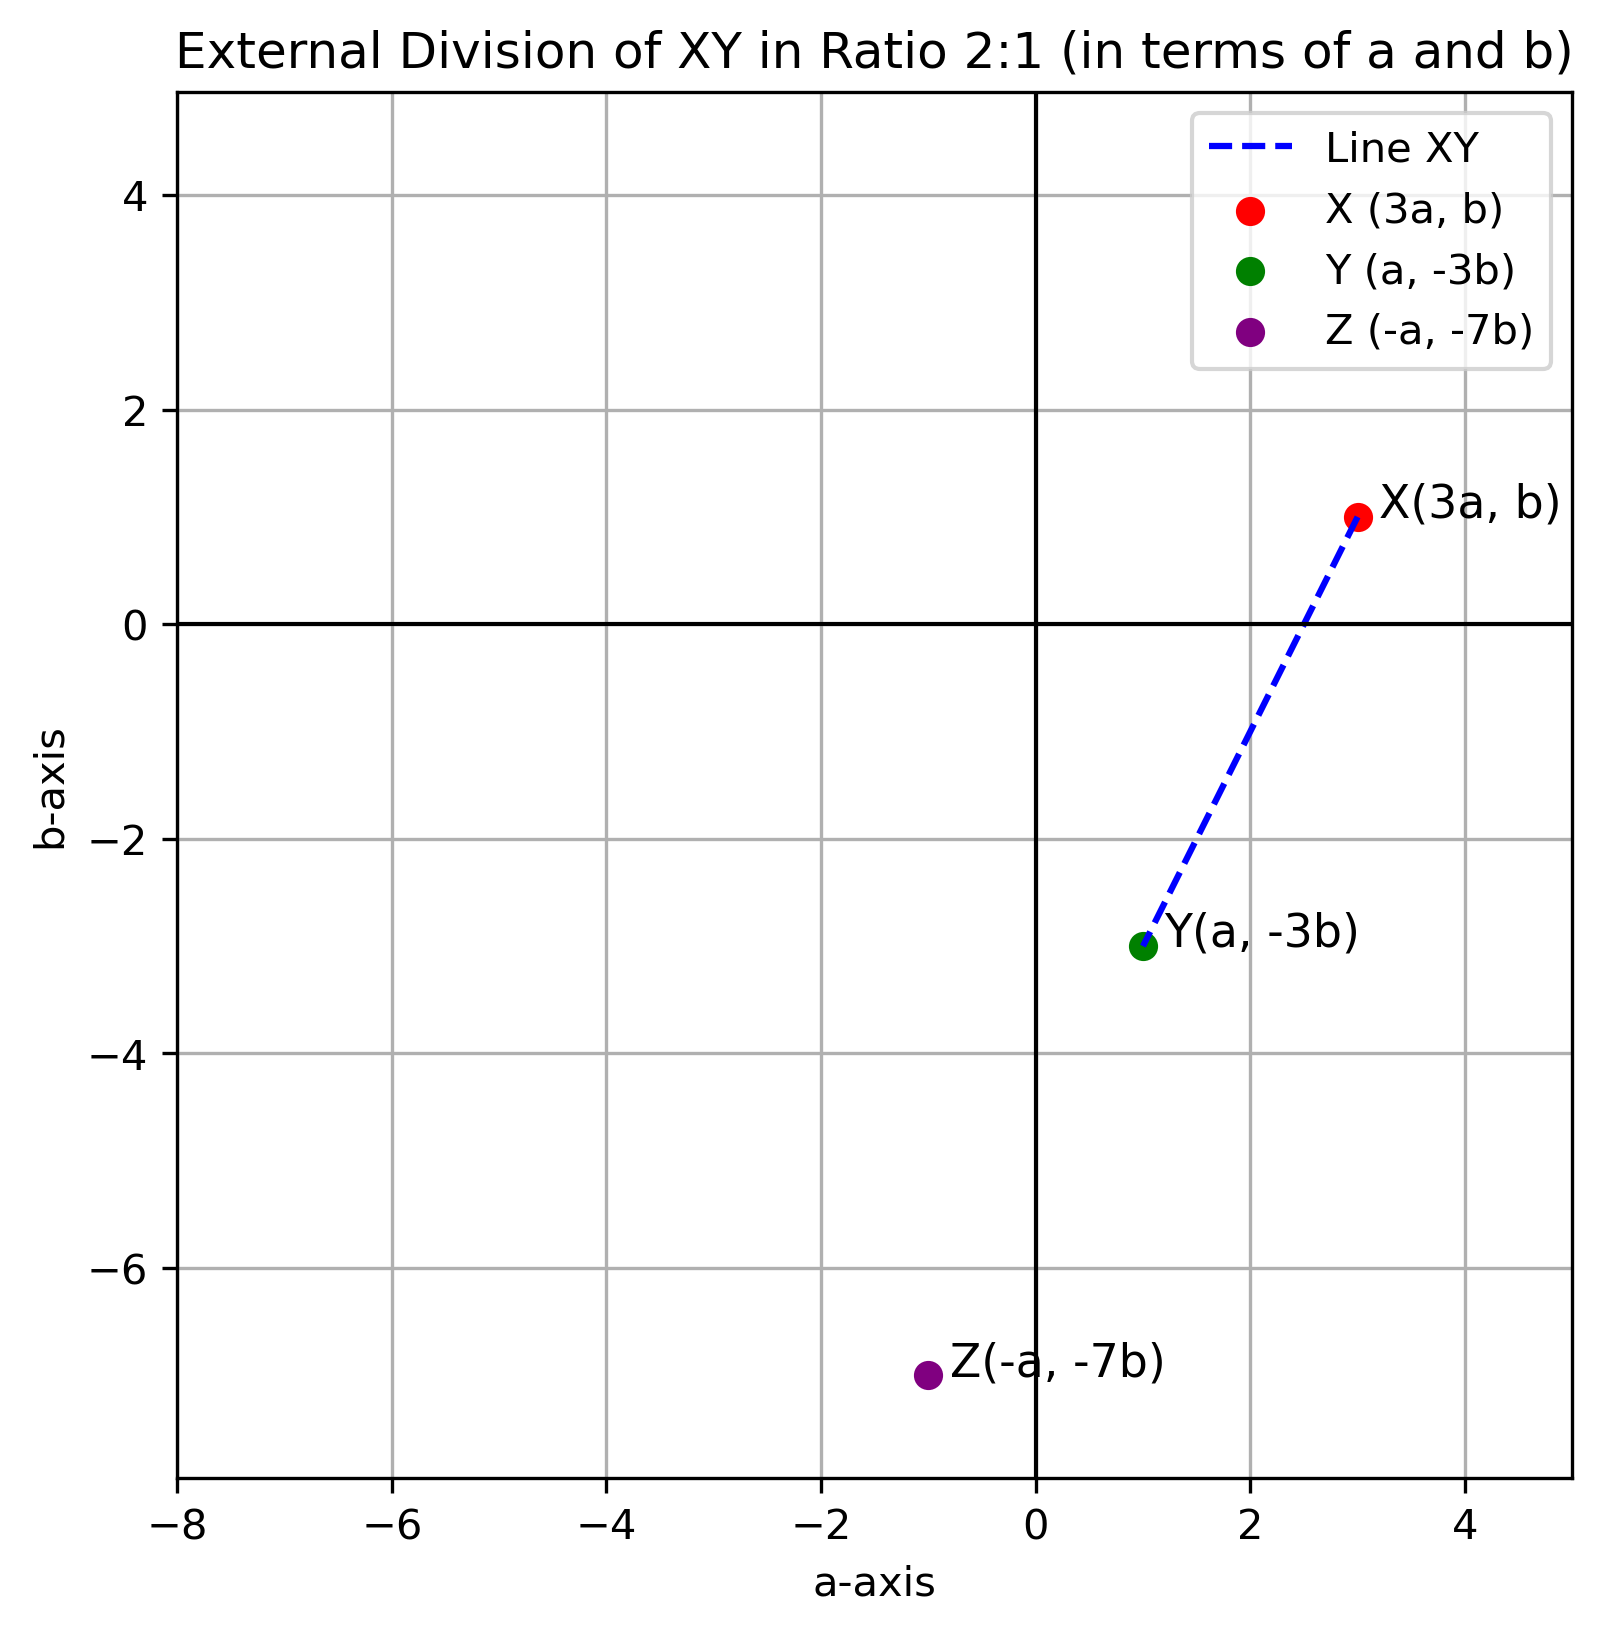
\includegraphics[width=0.8\linewidth]{figs/01.png}
    \caption{Caption}
    \label{fig:placeholder}
\end{figure}


\end{document}
